\batchmode
\documentclass[11pt]{article}
\RequirePackage{ifthen}


\usepackage[dvips]{graphicx}
\usepackage{times}

\graphicspath{{./}{figs/}}
\topmargin 0.0in
\textwidth 6.5in
\textheight 8.75in
\columnsep 0.25in
\oddsidemargin 0.0in
\evensidemargin 0.0in
\headsep 0.0in
\headheight 0.0in

\title{PVFS2 High-Availability Clustering}
\author{PVFS2 Development Team}\date{June, 2004}

\pagestyle{plain}


\usepackage[dvips]{color}


\pagecolor[gray]{.7}

\usepackage[]{inputenc}



\makeatletter

\makeatletter
\count@=\the\catcode`\_ \catcode`\_=8 
\newenvironment{tex2html_wrap}{}{}%
\catcode`\<=12\catcode`\_=\count@
\newcommand{\providedcommand}[1]{\expandafter\providecommand\csname #1\endcsname}%
\newcommand{\renewedcommand}[1]{\expandafter\providecommand\csname #1\endcsname{}%
  \expandafter\renewcommand\csname #1\endcsname}%
\newcommand{\newedenvironment}[1]{\newenvironment{#1}{}{}\renewenvironment{#1}}%
\let\newedcommand\renewedcommand
\let\renewedenvironment\newedenvironment
\makeatother
\let\mathon=$
\let\mathoff=$
\ifx\AtBeginDocument\undefined \newcommand{\AtBeginDocument}[1]{}\fi
\newbox\sizebox
\setlength{\hoffset}{0pt}\setlength{\voffset}{0pt}
\addtolength{\textheight}{\footskip}\setlength{\footskip}{0pt}
\addtolength{\textheight}{\topmargin}\setlength{\topmargin}{0pt}
\addtolength{\textheight}{\headheight}\setlength{\headheight}{0pt}
\addtolength{\textheight}{\headsep}\setlength{\headsep}{0pt}
\setlength{\textwidth}{349pt}
\newwrite\lthtmlwrite
\makeatletter
\let\realnormalsize=\normalsize
\global\topskip=2sp
\def\preveqno{}\let\real@float=\@float \let\realend@float=\end@float
\def\@float{\let\@savefreelist\@freelist\real@float}
\def\liih@math{\ifmmode$\else\bad@math\fi}
\def\end@float{\realend@float\global\let\@freelist\@savefreelist}
\let\real@dbflt=\@dbflt \let\end@dblfloat=\end@float
\let\@largefloatcheck=\relax
\let\if@boxedmulticols=\iftrue
\def\@dbflt{\let\@savefreelist\@freelist\real@dbflt}
\def\adjustnormalsize{\def\normalsize{\mathsurround=0pt \realnormalsize
 \parindent=0pt\abovedisplayskip=0pt\belowdisplayskip=0pt}%
 \def\phantompar{\csname par\endcsname}\normalsize}%
\def\lthtmltypeout#1{{\let\protect\string \immediate\write\lthtmlwrite{#1}}}%
\newcommand\lthtmlhboxmathA{\adjustnormalsize\setbox\sizebox=\hbox\bgroup\kern.05em }%
\newcommand\lthtmlhboxmathB{\adjustnormalsize\setbox\sizebox=\hbox to\hsize\bgroup\hfill }%
\newcommand\lthtmlvboxmathA{\adjustnormalsize\setbox\sizebox=\vbox\bgroup %
 \let\ifinner=\iffalse \let\)\liih@math }%
\newcommand\lthtmlboxmathZ{\@next\next\@currlist{}{\def\next{\voidb@x}}%
 \expandafter\box\next\egroup}%
\newcommand\lthtmlmathtype[1]{\gdef\lthtmlmathenv{#1}}%
\newcommand\lthtmllogmath{\lthtmltypeout{l2hSize %
:\lthtmlmathenv:\the\ht\sizebox::\the\dp\sizebox::\the\wd\sizebox.\preveqno}}%
\newcommand\lthtmlfigureA[1]{\let\@savefreelist\@freelist
       \lthtmlmathtype{#1}\lthtmlvboxmathA}%
\newcommand\lthtmlpictureA{\bgroup\catcode`\_=8 \lthtmlpictureB}%
\newcommand\lthtmlpictureB[1]{\lthtmlmathtype{#1}\egroup
       \let\@savefreelist\@freelist \lthtmlhboxmathB}%
\newcommand\lthtmlpictureZ[1]{\hfill\lthtmlfigureZ}%
\newcommand\lthtmlfigureZ{\lthtmlboxmathZ\lthtmllogmath\copy\sizebox
       \global\let\@freelist\@savefreelist}%
\newcommand\lthtmldisplayA{\bgroup\catcode`\_=8 \lthtmldisplayAi}%
\newcommand\lthtmldisplayAi[1]{\lthtmlmathtype{#1}\egroup\lthtmlvboxmathA}%
\newcommand\lthtmldisplayB[1]{\edef\preveqno{(\theequation)}%
  \lthtmldisplayA{#1}\let\@eqnnum\relax}%
\newcommand\lthtmldisplayZ{\lthtmlboxmathZ\lthtmllogmath\lthtmlsetmath}%
\newcommand\lthtmlinlinemathA{\bgroup\catcode`\_=8 \lthtmlinlinemathB}
\newcommand\lthtmlinlinemathB[1]{\lthtmlmathtype{#1}\egroup\lthtmlhboxmathA
  \vrule height1.5ex width0pt }%
\newcommand\lthtmlinlineA{\bgroup\catcode`\_=8 \lthtmlinlineB}%
\newcommand\lthtmlinlineB[1]{\lthtmlmathtype{#1}\egroup\lthtmlhboxmathA}%
\newcommand\lthtmlinlineZ{\egroup\expandafter\ifdim\dp\sizebox>0pt %
  \expandafter\centerinlinemath\fi\lthtmllogmath\lthtmlsetinline}
\newcommand\lthtmlinlinemathZ{\egroup\expandafter\ifdim\dp\sizebox>0pt %
  \expandafter\centerinlinemath\fi\lthtmllogmath\lthtmlsetmath}
\newcommand\lthtmlindisplaymathZ{\egroup %
  \centerinlinemath\lthtmllogmath\lthtmlsetmath}
\def\lthtmlsetinline{\hbox{\vrule width.1em \vtop{\vbox{%
  \kern.1em\copy\sizebox}\ifdim\dp\sizebox>0pt\kern.1em\else\kern.3pt\fi
  \ifdim\hsize>\wd\sizebox \hrule depth1pt\fi}}}
\def\lthtmlsetmath{\hbox{\vrule width.1em\kern-.05em\vtop{\vbox{%
  \kern.1em\kern0.8 pt\hbox{\hglue.17em\copy\sizebox\hglue0.8 pt}}\kern.3pt%
  \ifdim\dp\sizebox>0pt\kern.1em\fi \kern0.8 pt%
  \ifdim\hsize>\wd\sizebox \hrule depth1pt\fi}}}
\def\centerinlinemath{%
  \dimen1=\ifdim\ht\sizebox<\dp\sizebox \dp\sizebox\else\ht\sizebox\fi
  \advance\dimen1by.5pt \vrule width0pt height\dimen1 depth\dimen1 
 \dp\sizebox=\dimen1\ht\sizebox=\dimen1\relax}

\def\lthtmlcheckvsize{\ifdim\ht\sizebox<\vsize 
  \ifdim\wd\sizebox<\hsize\expandafter\hfill\fi \expandafter\vfill
  \else\expandafter\vss\fi}%
\providecommand{\selectlanguage}[1]{}%
\makeatletter \tracingstats = 1 


\begin{document}
\pagestyle{empty}\thispagestyle{empty}\lthtmltypeout{}%
\lthtmltypeout{latex2htmlLength hsize=\the\hsize}\lthtmltypeout{}%
\lthtmltypeout{latex2htmlLength vsize=\the\vsize}\lthtmltypeout{}%
\lthtmltypeout{latex2htmlLength hoffset=\the\hoffset}\lthtmltypeout{}%
\lthtmltypeout{latex2htmlLength voffset=\the\voffset}\lthtmltypeout{}%
\lthtmltypeout{latex2htmlLength topmargin=\the\topmargin}\lthtmltypeout{}%
\lthtmltypeout{latex2htmlLength topskip=\the\topskip}\lthtmltypeout{}%
\lthtmltypeout{latex2htmlLength headheight=\the\headheight}\lthtmltypeout{}%
\lthtmltypeout{latex2htmlLength headsep=\the\headsep}\lthtmltypeout{}%
\lthtmltypeout{latex2htmlLength parskip=\the\parskip}\lthtmltypeout{}%
\lthtmltypeout{latex2htmlLength oddsidemargin=\the\oddsidemargin}\lthtmltypeout{}%
\makeatletter
\if@twoside\lthtmltypeout{latex2htmlLength evensidemargin=\the\evensidemargin}%
\else\lthtmltypeout{latex2htmlLength evensidemargin=\the\oddsidemargin}\fi%
\lthtmltypeout{}%
\makeatother
\setcounter{page}{1}
\onecolumn

% !!! IMAGES START HERE !!!

\stepcounter{section}
\stepcounter{section}
\stepcounter{section}
\stepcounter{subsection}
{\newpage\clearpage
\lthtmlinlinemathA{tex2html_wrap_inline141}%
$\rightarrow$%
\lthtmlinlinemathZ
\lthtmlcheckvsize\clearpage}

\stepcounter{subsection}
\stepcounter{subsection}
\stepcounter{subsubsection}
{\newpage\clearpage
\lthtmlpictureA{tex2html_wrap478}%
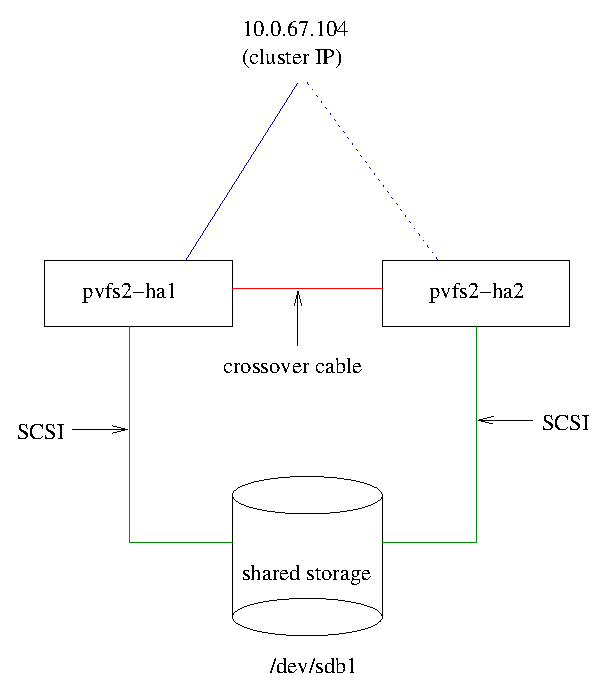
\includegraphics[scale=0.75]{pvfs2-failover.eps}%
\lthtmlpictureZ
\lthtmlcheckvsize\clearpage}

{\newpage\clearpage
\lthtmlfigureA{figure46}%
\begin{figure}\begin{scriptsize}
\begin{verbatim}

# pretty self explanatory: send heartbeat logging to the /var/log/ha-log
# file and also syslog with the 'local0' level
logfile /var/log/ha-log
logfacility local0

# we are using a network cable for our primary (and only) heartbeat
# channel.  It also might be a good idea to use a serial cable for a
# secondary channel.  Since we are aiming for high-availability, the
# more heartbeat channels the better.  The ha.cf and GettingStarted
# files document how to set up other heartbeat channels.
bcast eth1

# When a service runs on A, then A dies and B takes over, do you want A
# to take it back (auto failback) from B when it recovers?  
auto_failback on

# here is where you tell heartbeat the names (uname -n) of the
# nodes in this cluster.
node pvfs2-ha1
node pvfs2-ha2

# heartbeat needs to know the difference between it's partner node
# dieing and the entire network failing up, so give it the IP address of
# a stable machine (e.g. a router) in your network.
ping 10.0.67.253

# the 'ipfail' program keeps an eye on the network
respawn hacluster /usr/lib/heartbeat/ipfail\end{verbatim}
\end{scriptsize}
\end{figure}%
\lthtmlfigureZ
\lthtmlcheckvsize\clearpage}

{\newpage\clearpage
\lthtmlfigureA{figure54}%
\begin{figure}\begin{scriptsize}
\begin{verbatim}

# this line describes resources managed by heartbeat.  
#   pvfs2-ha1: the primary host for this service.  Heartbeat will start
#              these resources on pvfs2-ha1 if that node is up
#   10.0.67.104: the 'cluster' (or shared) IP address for these
#              nodes. refer to the comments in haresources for the many
#              many options you can use to express network settings. 
#   Filesystem::/dev/sdb3::/shared::ext3
#              Describes a 'filesystem' resource.  '::' delimits
#              arguments.  <device>::<mount point>::<fs type>
#   pvfs2:     the service.  heartbeat will look for, in this order
#              /etc/ha.d/resource.d/pvfs2 
#              /etc/init.d/pvfs2
#              When starting, heartbeat will call 'pvfs2 start'
#              When nicely shutting down, will call 'pvfs2 stop'
#              so make sure the script understands those arguments.
#              Typical service init scripts work great.
pvfs2-ha1 10.0.67.104 Filesystem::/dev/sdb3::/shared::ext3 pvfs2\end{verbatim}
\end{scriptsize}
\end{figure}%
\lthtmlfigureZ
\lthtmlcheckvsize\clearpage}

{\newpage\clearpage
\lthtmlfigureA{figure62}%
\begin{figure}\begin{scriptsize}
\begin{verbatim}

# you can specify multiple authentication methods, each prefixed with a
# 'method-id'. 'auth 1' means use method-id 1
auth 1

# and here's the entry for method-id 1:
# crc is the weakest of the hashes, and should only be used over secure
# links... like a crossover cable.   If you were sending heartbeat over
# an insecure channel or through routers, you would use a stronger hash
# to prevent man-in-the-middle attacks on the heartbeat nodes.
1 crc\end{verbatim}
\end{scriptsize}
\end{figure}%
\lthtmlfigureZ
\lthtmlcheckvsize\clearpage}

{\newpage\clearpage
\lthtmlfigureA{figure70}%
\begin{figure}\begin{scriptsize}
\begin{verbatim}

eth0      Link encap:Ethernet  HWaddr 00:0F:1F:6A:6F:DC  
          inet addr:10.0.67.105  Bcast:140.221.67.255  Mask:255.255.254.0
          UP BROADCAST RUNNING MULTICAST  MTU:1500  Metric:1
          RX packets:2893591 errors:0 dropped:0 overruns:0 frame:0
          TX packets:1637691 errors:0 dropped:0 overruns:0 carrier:0
          collisions:0 txqueuelen:1000 
          RX bytes:1304753410 (1.2 GiB)  TX bytes:189439176 (180.6 MiB)
          Interrupt:28 

eth0:0    Link encap:Ethernet  HWaddr 00:0F:1F:6A:6F:DC  
          inet addr:10.0.67.104  Bcast:140.221.67.255  Mask:255.255.254.0
          UP BROADCAST RUNNING MULTICAST  MTU:1500  Metric:1
          Interrupt:28 

eth1      Link encap:Ethernet  HWaddr 00:0F:1F:6A:6F:DD  
          inet addr:192.168.1.1  Bcast:192.168.1.255  Mask:255.255.255.0
          UP BROADCAST RUNNING MULTICAST  MTU:1500  Metric:1
          RX packets:1188003 errors:0 dropped:0 overruns:0 frame:0
          TX packets:944704 errors:0 dropped:0 overruns:0 carrier:0
          collisions:0 txqueuelen:1000 
          RX bytes:197055953 (187.9 MiB)  TX bytes:156677942 (149.4 MiB)
          Interrupt:29\end{verbatim}
\end{scriptsize}
\end{figure}%
\lthtmlfigureZ
\lthtmlcheckvsize\clearpage}

\stepcounter{subsubsection}
{\newpage\clearpage
\lthtmlpictureA{tex2html_wrap495}%
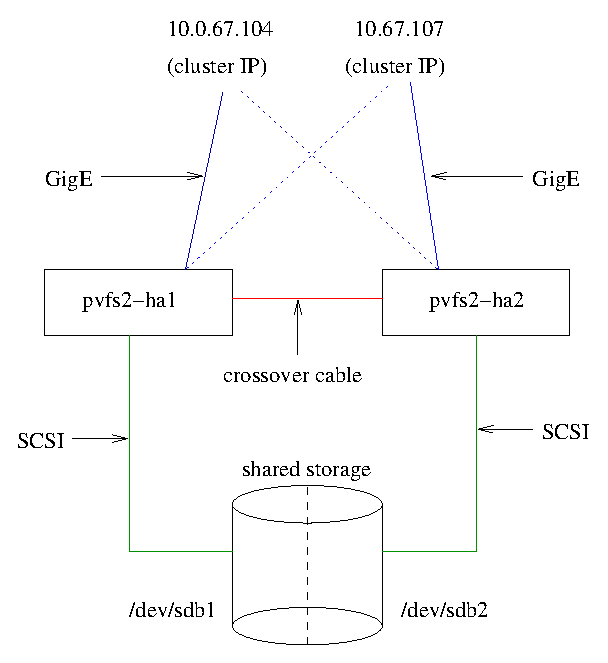
\includegraphics[scale=0.75]{pvfs2-failover-AA.eps}%
\lthtmlpictureZ
\lthtmlcheckvsize\clearpage}

{\newpage\clearpage
\lthtmlfigureA{figure99}%
\begin{figure}\begin{scriptsize}
\begin{verbatim}

PVFS2_FS_CONF=/etc/pvfs2/fs.conf
PVFS2_SERVER_CONF=/etc/pvfs2/server.conf-140.221.67.104
        
# override this if your server binary resides elsewhere
PVFS2SERVER=/usr/local/sbin/pvfs2-server
# override this if you want servers to automatically pick a conf file,
#   but you just need to specify what directory they are in
PVFS2_CONF_PATH=/etc/pvfs2
PVFS2_PIDFILE=/var/run/pvfs2-1.pid
...  # remainder of init script omitted\end{verbatim}
\end{scriptsize}
\end{figure}%
\lthtmlfigureZ
\lthtmlcheckvsize\clearpage}

{\newpage\clearpage
\lthtmlfigureA{figure107}%
\begin{figure}\begin{scriptsize}
\begin{verbatim}

PVFS2_FS_CONF=/etc/pvfs2/fs.conf
PVFS2_SERVER_CONF=/etc/pvfs2/server.conf-140.221.67.107
        
# override this if your server binary resides elsewhere
PVFS2SERVER=/usr/local/sbin/pvfs2-server
# override this if you want servers to automatically pick a conf file,
#   but you just need to specify what directory they are in
PVFS2_CONF_PATH=/etc/pvfs2
PVFS2_PIDFILE=/var/run/pvfs2-2.pid
...  # remainder of init script omitted\end{verbatim}
\end{scriptsize}
\end{figure}%
\lthtmlfigureZ
\lthtmlcheckvsize\clearpage}

{\newpage\clearpage
\lthtmlfigureA{figure115}%
\begin{figure}\begin{scriptsize}
\begin{verbatim}

# Each server has its associated IP address and file system.  pvfs2-1,
# for example,  is associated with 10.0.67.104 and has its data on
# sdb1.  
# 
# note that each server has its own file system.  You must have a
# dedicated partition for each service you run via heartbeat.

pvfs2-ha1 10.0.67.104 Filesystem::/dev/sdb1::/mnt/shared1::ext3 pvfs2-1
pvfs2-ha2 10.0.67.107 Filesystem::/dev/sdb2::/mnt/shared2::ext3 pvfs2-2\end{verbatim}
\end{scriptsize}
\end{figure}%
\lthtmlfigureZ
\lthtmlcheckvsize\clearpage}

{\newpage\clearpage
\lthtmlfigureA{figure125}%
\begin{figure}\begin{scriptsize}
\begin{verbatim}

eth0      Link encap:Ethernet  HWaddr 00:0F:1F:6A:6F:DC  
          inet addr:140.221.67.105  Bcast:140.221.67.255  Mask:255.255.254.0
          UP BROADCAST RUNNING MULTICAST  MTU:1500  Metric:1
          RX packets:2911950 errors:0 dropped:0 overruns:0 frame:0
          TX packets:1647984 errors:0 dropped:0 overruns:0 carrier:0
          collisions:0 txqueuelen:1000 
          RX bytes:1306604241 (1.2 GiB)  TX bytes:190743053 (181.9 MiB)
          Interrupt:28 

eth0:0    Link encap:Ethernet  HWaddr 00:0F:1F:6A:6F:DC  
          inet addr:140.221.67.104  Bcast:140.221.67.255  Mask:255.255.254.0
          UP BROADCAST RUNNING MULTICAST  MTU:1500  Metric:1
          Interrupt:28 

eth0:1    Link encap:Ethernet  HWaddr 00:0F:1F:6A:6F:DC  
          inet addr:140.221.67.107  Bcast:140.221.67.255  Mask:255.255.254.0
          UP BROADCAST RUNNING MULTICAST  MTU:1500  Metric:1
          Interrupt:28 

eth1      Link encap:Ethernet  HWaddr 00:0F:1F:6A:6F:DD  
          inet addr:192.168.1.1  Bcast:192.168.1.255  Mask:255.255.255.0
          UP BROADCAST RUNNING MULTICAST  MTU:1500  Metric:1
          RX packets:1197984 errors:0 dropped:0 overruns:0 frame:0
          TX packets:954689 errors:0 dropped:0 overruns:0 carrier:0
          collisions:0 txqueuelen:1000 
          RX bytes:198722216 (189.5 MiB)  TX bytes:158334802 (150.9 MiB)
          Interrupt:29\end{verbatim}
\end{scriptsize}
\end{figure}%
\lthtmlfigureZ
\lthtmlcheckvsize\clearpage}

\stepcounter{section}

\end{document}
